\section{Resultados e discussão}
\label{sec:resultados}

%=====================================================================
\subsection{FRFs experimentais}
\label{sec:frf_exp}

\subsubsection{Ensaio com martelo}

A Figura~\ref{fig:frf_martelo} mostra a acelerância do ensaio com martelo, com módulo,
fase e coerência. Aparecem seis picos de flexão na faixa medida, em \num{25.2}; \num{164.1};
\num{459.0}; \num{893.2}; \num{1462.3} e \SI{2157.5}{\hertz}. Os
estimadores $H_1$ e $H_2$ praticamente coincidem onde a coerência é próxima de 1 e
só se separam nas antirressonâncias e abaixo de \SI{20}{\hertz}, onde a resposta é
pequena e o ruído pesa mais; nessas faixas a coerência cai, como esperado. Os picos
têm coerência acima de \num{0.96}, com duas exceções: o modo 3 (\num{0.84}), que é
fraco porque o ponto de impacto fica muito perto de um nó desse modo
(Figura~\ref{fig:modos}), e o modo 5 (\num{0.60}), vizinho de uma antirressonância
em torno de \SI{1.5}{\kilo\hertz}.

\begin{figure}[htbp]
    \centering
    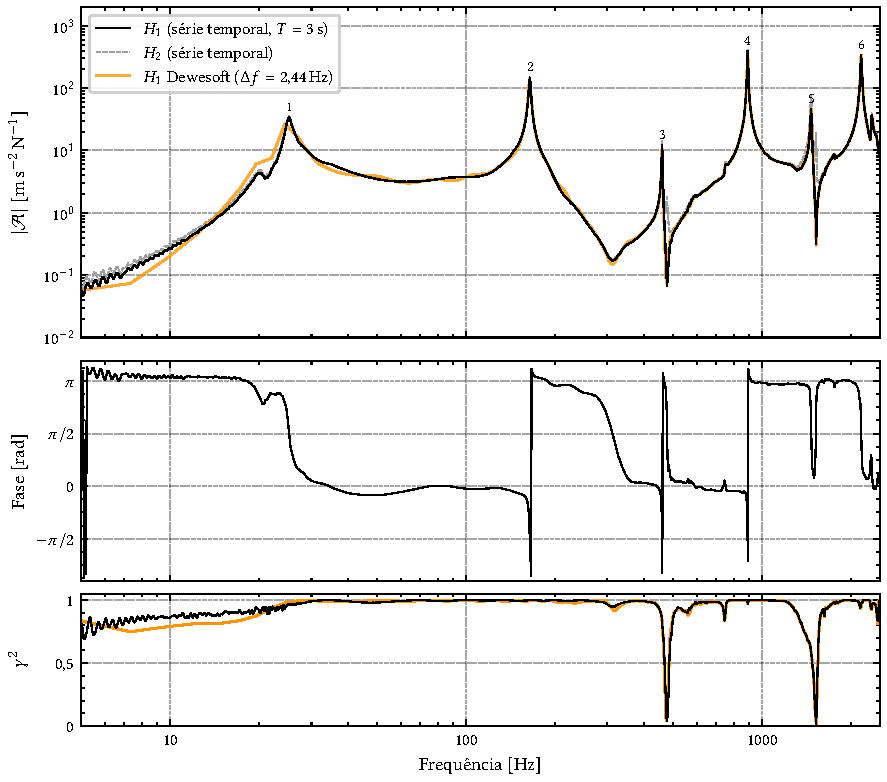
\includegraphics[width=\textwidth]{frf_martelo.pdf}
    \caption{Acelerância $\ddot w(x_e)/f(x_i)$ do ensaio com martelo ($x_i =
            \SI{0.200}{\meter}$, $x_e = \SI{0.356}{\meter}$): módulo, fase de $H_1$ e
        coerência. Em preto e cinza, $H_1$ e $H_2$ recalculados da série temporal; em
        laranja, $H_1$ exportado pelo Dewesoft. Os números indicam os modos de flexão.}
    \label{fig:frf_martelo}
\end{figure}

A curva exportada pelo Dewesoft concorda com a recalculada em quase toda a faixa,
mas não no primeiro modo, em que o pico fica mais baixo e mais largo. A
Tabela~\ref{tab:resolucao} quantifica a diferença. Com $\Delta f = \SI{2.44}{\hertz}$
e registros de \SI{0.41}{\second}, a banda de meia potência do modo 1 contém um único
ponto, e a meia potência dá $\zeta_1 = \SI{6.1}{\percent}$; com a FRF recalculada,
há 32 pontos na banda e $\zeta_1 = \SI{2.40}{\percent}$. A partir do modo 2 as duas
estimativas de frequência diferem menos de \SI{1}{\hertz}, e as de amortecimento
convergem à medida que a banda passa a conter mais pontos. As frequências e
amortecimentos do martelo usados daqui em diante são os da FRF recalculada.

\begin{table}[htbp]
    \centering
    \caption{Ensaio com martelo: parâmetros modais obtidos da FRF exportada pelo
        Dewesoft e da FRF recalculada a partir da série temporal. $n$ é o número de
        pontos dentro da banda de meia potência.}
    \label{tab:resolucao}
    \begin{tabular}{c rrr rrrr}
        \toprule
             & \multicolumn{3}{c}{Dewesoft ($\Delta f = \SI{2.44}{\hertz}$)}
             & \multicolumn{4}{c}{Série temporal ($T = \SI{3}{\second}$)}                                                    \\
        \cmidrule(lr){2-4}\cmidrule(lr){5-8}
        Modo & $f_r$ [\si{\hertz}] & $\zeta_r$ [\si{\percent}] & $n$
             & $f_r$ [\si{\hertz}] & $\zeta_r$ [\si{\percent}] & $n$ & $\gamma^2$                                          \\
        \midrule
        \linhas{martelo_resolucao}
        \bottomrule
    \end{tabular}
\end{table}

A fase confirma a identificação dos modos. Numa FRF de transferência, cada modo
contribui com $W_r(x_e)W_r(x_i)/(\omega_r^2 - \Omega^2 + 2\iu\zeta_r\omega_r\Omega)$,
e a fase da acelerância na ressonância é $+\pi/2$ se a constante modal
$W_r(x_e)W_r(x_i)$ for positiva e $-\pi/2$ se for negativa. Os modos 1, 5 e 6 passam
por $+\pi/2$ e os modos 2, 3 e 4 por $-\pi/2$. Essa sequência é comparada com os
modelos na Seção~\ref{sec:molas_res}. Há ainda um pequeno pico em
\SI{20.3}{\hertz}, abaixo do primeiro modo, que não corresponde a nenhum modo de
flexão da viga; ele reaparece no ensaio com \emph{shaker} e é discutido adiante.

\subsubsection{Ensaio com \emph{shaker}}

A Figura~\ref{fig:frf_shaker} mostra a acelerância pontual medida na ponta. Como
força e aceleração são medidas no mesmo ponto, todas as constantes modais
$W_r(L)^2$ são positivas: ressonâncias e antirressonâncias se alternam e a fase fica
entre 0 e $\pi$, passando por $\pi/2$ em cada ressonância \cite{ewins2000}. Os dados
seguem esse padrão. Há quatro picos associados a modos de flexão (\num{24.1}; \num{160.8};
\num{495.5} e \SI{966.8}{\hertz}) e um quinto, em \SI{387.4}{\hertz} (marcado com ``?''), que forma
um par quase coincidente com uma antirressonância em \SI{383}{\hertz} e não tem
correspondente no ensaio com martelo nem nos modelos. Um par polo--zero tão próximo
indica um modo que quase não participa da resposta na ponta; é provável que venha do
conjunto \emph{shaker}--haste ou de um modo que não é de flexão vertical (torção ou
flexão lateral) excitado por algum desalinhamento. Esse pico foi excluído da comparação
com os modelos.

\begin{figure}[htbp]
    \centering
    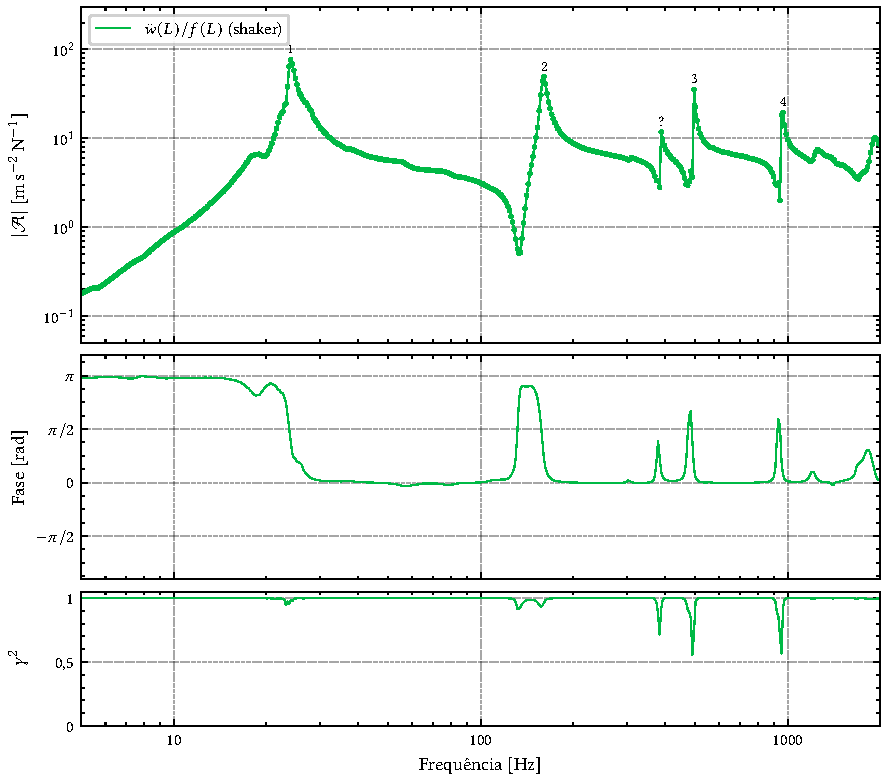
\includegraphics[width=\textwidth]{frf_shaker.pdf}
    \caption{Acelerância pontual $\ddot w(L)/f(L)$ do ensaio com \emph{shaker}: módulo,
        fase e coerência. Os pontos são as 512 frequências da varredura.}
    \label{fig:frf_shaker}
\end{figure}

Nos dois ensaios aparece também uma pequena ressonância isolada abaixo do primeiro
modo, em \SI{20.3}{\hertz} no martelo e em torno de \SI{19}{\hertz} no
\emph{shaker}, com uma perturbação localizada na fase. Ela não é prevista por nenhum
modelo da viga, e sua presença nas duas montagens, com excitações diferentes, sugere
um modo da estrutura de suporte. Isso é um indício direto de que a base não é
perfeitamente rígida.

%=====================================================================
\subsection{Frequências naturais e amortecimento: martelo \texorpdfstring{$\times$}{x} \emph{shaker}}
\label{sec:comparacao_ensaios}

A Tabela~\ref{tab:martelo_shaker} compara os parâmetros modais dos dois ensaios.

\begin{table}[htbp]
    \centering
    \caption{Frequências naturais e fatores de amortecimento identificados nos dois
        ensaios. $n$ é o número de pontos medidos na banda de meia potência do
        \emph{shaker}, e $\Delta f$, a diferença relativa entre as frequências do
        \emph{shaker} e do martelo.}
    \label{tab:martelo_shaker}
    \begin{tabular}{c rr rrrr r}
        \toprule
             & \multicolumn{2}{c}{Martelo} & \multicolumn{4}{c}{\emph{Shaker}} &                                                   \\
        \cmidrule(lr){2-3}\cmidrule(lr){4-7}
        Modo & $f_r$ [\si{\hertz}]         & $\zeta_r$ [\si{\percent}]         & $f_r$ [\si{\hertz}] & $\zeta_r$ [\si{\percent}]
             & $n$                         & $\gamma^2$                        & $\Delta f$ [\si{\percent}]                         \\
        \midrule
        \linhas{martelo_shaker}
        \bottomrule
    \end{tabular}
\end{table}

\paragraph{Frequências.} Os dois primeiros modos do \emph{shaker} ficam
\SI{4.6}{\percent} e \SI{2.0}{\percent} abaixo dos do martelo, enquanto os modos 3 e 4
ficam cerca de \SI{8}{\percent} acima. As duas montagens não são, portanto, o mesmo
sistema. No ensaio com \emph{shaker}, a cabeça de impedância e sua fixação acrescentam
massa à ponta, o que reduz as frequências. Usando o modelo com base elástica ajustado
na Seção~\ref{sec:molas_res}, uma massa de \SI{17}{\gram} na ponta reproduziria a
queda do modo 1, mas também reduziria os modos 2, 3 e 4 em \SI{4.3}{\percent},
\SI{3.9}{\percent} e \SI{3.3}{\percent}. Como os modos 3 e 4 medidos sobem, a ligação
deve também restringir a ponta: a haste e a cabeça de impedância transmitem momento e
dificultam a rotação da extremidade, o que enrijece sobretudo os modos mais altos,
cuja forma tem grande rotação na ponta. A célula de carga mede só a força axial da
haste; o momento transmitido não entra na FRF medida, de modo que esse efeito aparece
como uma mudança no próprio sistema ensaiado. Por isso o ensaio com martelo, com a
ponta realmente livre, é a referência para o ajuste do modelo.

\paragraph{Amortecimento.} No martelo, o primeiro modo tem
$\zeta_1 = \SI{2.40}{\percent}$, bem mais que os demais
(\SIrange{0.20}{0.61}{\percent}). O \emph{shaker} confirma esse valor
($\zeta_1 = \SI{2.21}{\percent}$, com 4 pontos na banda), mas dá amortecimentos 3 a 6
vezes maiores nos modos 2 a 4. Esses valores do \emph{shaker} não são confiáveis: com
passo de \SI{1.18}{\percent}, a banda de meia potência desses modos contém de 1 a 3
pontos, o ponto mais alto medido fica, em geral, abaixo do pico real, e a banda
estimada resulta mais larga. Além disso, na ressonância a impedância da viga na ponta
é mínima e o \emph{shaker} consegue impor pouca força, o que reduz a relação
sinal--ruído justamente no pico (a coerência do modo 3, \num{0.73}, é a mais baixa).
Os fatores do martelo, obtidos com dezenas a centenas de pontos por banda, são
adotados como representativos da viga. O amortecimento maior do modo 1 é compatível
com dissipação no engaste parafusado: no modelo ajustado na
Seção~\ref{sec:molas_res}, é no modo 1 que a mola torcional da base armazena a maior
parcela da energia de deformação (\SI{35}{\percent}, contra no máximo
\SI{17}{\percent} nos demais modos). Também pode contribuir a troca de energia com o
modo do suporte em torno de \SI{20}{\hertz}, vizinho de $f_1$. Os dados não permitem
separar essas contribuições.

%=====================================================================
\subsection{Efeito da massa na ponta}
\label{sec:massa}

Os ensaios foram feitos sem a massa concentrada de \SI{0.445}{\kilo\gram}. Para
avaliar quanto as frequências teriam mudado com ela, os dois modelos foram resolvidos
com $\mu = \num{0.705}$, mantendo as mesmas condições na base: o engaste ideal e a base
elástica ajustada na Seção~\ref{sec:molas_res}. A Tabela~\ref{tab:massa} e a
Figura~\ref{fig:massa} mostram o resultado.

\begin{table}[htbp]
    \centering
    \caption{Frequências naturais [\si{\hertz}] sem massa ($\mu = 0$) e com a massa de
        \SI{0.445}{\kilo\gram} na ponta ($\mu = \num{0.705}$), para as duas condições de
        base, e variação relativa causada pela massa.}
    \label{tab:massa}
    \begin{tabular}{c r rrr rrr}
        \toprule
             &          & \multicolumn{3}{c}{Base engastada} & \multicolumn{3}{c}{Base elástica ajustada}                                                                        \\
        \cmidrule(lr){3-5}\cmidrule(lr){6-8}
        Modo & Medido   & $\mu = 0$                          & $\mu = \num{0.705}$                        & Var. [\si{\percent}] & $\mu = 0$ & $\mu = \num{0.705}$ & Var. [\si{\percent}] \\
        \midrule
        \linhas{massa_ponta}
        \bottomrule
    \end{tabular}
\end{table}

\begin{figure}[htbp]
    \centering
    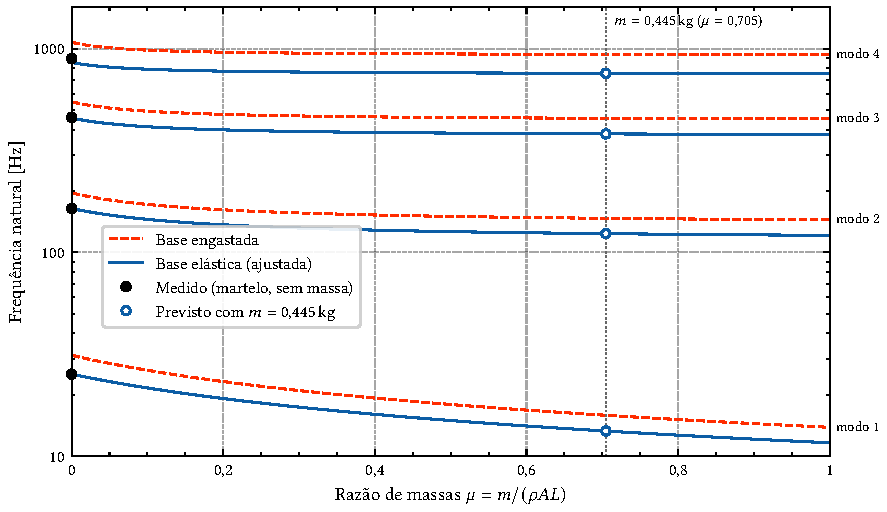
\includegraphics[width=\textwidth]{massa_ponta.pdf}
    \caption{Frequências naturais dos quatro primeiros modos em função da razão de
        massas $\mu$, para a base engastada e para a base elástica ajustada. Os pontos
        cheios são as frequências medidas (sem massa); os vazados, as previstas com a
        massa de \SI{0.445}{\kilo\gram}.}
    \label{fig:massa}
\end{figure}

Com a massa, o primeiro modo cairia quase pela metade, para \SI{15.8}{\hertz} com
engaste ideal e \SI{13.3}{\hertz} com a base elástica, e o segundo cairia
\SI{25}{\percent}, para \num{146.8} e \SI{123.4}{\hertz}. O efeito diminui nos modos
mais altos (\SIrange{8}{17}{\percent} nos modos 3 a 6). A massa fica onde todos os
modos têm amplitude máxima, mas seu efeito depende de quanto ela pesa em relação à
massa que participa de cada modo. No modo 1 a viga inteira se move em fase, e a massa
modal efetiva na ponta é cerca de um quarto da massa da viga, bem menor que
\SI{0.445}{\kilo\gram}. Nos modos altos, a massa grande praticamente impede a
translação da ponta, e as curvas da Figura~\ref{fig:massa} tendem aos modos de uma
viga engastada-apoiada: com $\mu \to \infty$, o modo $r$ tende ao modo $r - 1$ dessa
viga ($\lambda = \num{3.927}$; $\num{7.069}$; $\num{10.21}$; \dots), o que explica o
achatamento das curvas.

A comparação também confirma que o ensaio foi feito sem a massa. Qualquer
flexibilidade na base só reduz as frequências, de modo que o engaste ideal dá o maior
valor possível para cada modo. Com a massa, esse limite seria \SI{15.8}{\hertz} para
o modo 1 e \SI{146.8}{\hertz} para o modo 2, e o medido é \num{25.2} e
\SI{164.1}{\hertz}, acima dos dois limites. Os modos 3 e 4 do engaste com massa
(\num{454.7} e \SI{936.7}{\hertz}) ficam próximos dos medidos (\num{459.0} e
\SI{893.2}{\hertz}), mas isso é coincidência: são justamente os modos menos sensíveis
à massa, e não servem para discriminar as hipóteses. Os modos 1 e 2, os mais sensíveis,
são incompatíveis com ela.

%=====================================================================
\subsection{Condição de contorno: engaste ideal \texorpdfstring{$\times$}{x} base elástica}
\label{sec:molas_res}

\subsubsection{Engaste ideal}

O modelo engastado superestima todas as frequências medidas, de \SI{19}{\percent} a
\SI{24}{\percent} (Tabela~\ref{tab:validacao}). A FRF analítica correspondente
(Figura~\ref{fig:frf_martelo_modelos}) tem a forma certa, com a mesma sequência de
picos e antirressonâncias, mas deslocada para a direita, e fica abaixo da medida em
baixa frequência: a viga real é mais flexível que uma viga perfeitamente engastada.

\subsubsection{Ajuste da base elástica}

Resolvendo \eqref{eq:ajuste} com $f_{1,\mathrm{med}} = \SI{25.22}{\hertz}$ e
$f_{2,\mathrm{med}} = \SI{164.07}{\hertz}$, obtém-se
\begin{equation}
    \kappa_R = \vkapR, \qquad \kappa_L = \vkapL,
    \label{eq:molas_ajustadas}
\end{equation}
ou, em unidades físicas,
$k_R = \kappa_R EI/L = \SI{2.79e3}{\newton\meter\per\radian}$ e
$k_L = \kappa_L EI/L^3 = \SI{2.84e6}{\newton\per\meter}$.
A Figura~\ref{fig:ajuste} mostra o problema de ajuste no plano
$(\log_{10}\kappa_R, \log_{10}\kappa_L)$. As curvas $f_1 = f_{1,\mathrm{med}}$ e
$f_2 = f_{2,\mathrm{med}}$ se cruzam em um único ponto da região explorada. Para
$\kappa_L$ grande as duas ficam quase verticais, isto é, passam a depender só de
$\kappa_R$, e elas se cruzam com um ângulo pequeno. Na solução, uma década em
$\kappa_R$ muda $f_1$ em \SI{40}{\percent} e $f_2$ em \SI{19}{\percent}, enquanto uma
década em $\kappa_L$ muda $f_1$ em apenas \SI{0.4}{\percent} e $f_2$ em
\SI{5.4}{\percent}. Por isso $\kappa_R$ fica bem determinado, mas $\kappa_L$ não: uma
variação de \SI{1}{\percent} em $f_2$ leva $\kappa_L$ de cerca de \num{1000} a
\num{2600} (Tabela~\ref{tab:sensibilidade}). O ajuste com os dois primeiros picos do
\emph{shaker} dá $\kappa_R = \vkapRs$ e $\kappa_L = \vkapLs$: o mesmo $\kappa_L$
dentro dessa incerteza e um $\kappa_R$ menor, coerente com o $f_1$ do \emph{shaker}
rebaixado pela massa da cabeça de impedância.

\begin{figure}[htbp]
    \centering
    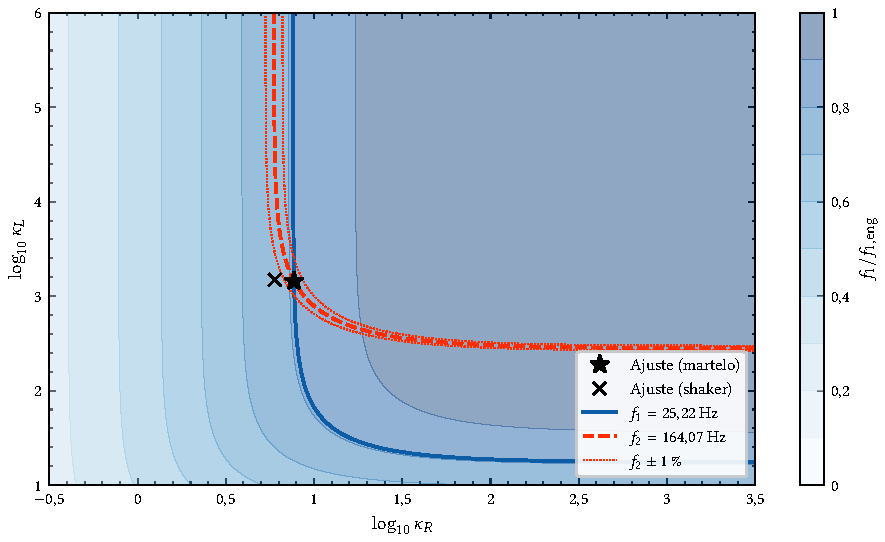
\includegraphics[width=\textwidth]{ajuste_molas.pdf}
    \caption{Ajuste da base elástica. Curvas de $f_1$ e $f_2$ iguais às medidas no
        martelo, no plano das rigidezes adimensionais; as linhas pontilhadas
        correspondem a $f_2 \pm \SI{1}{\percent}$. O fundo mostra $f_1$ relativo ao
        engaste ideal.}
    \label{fig:ajuste}
\end{figure}

O valor de $\kappa_R$ diz que a fixação tem rigidez à rotação de apenas
$\num{7.7}\,EI/L$. Estaticamente, a flexibilidade na ponta de uma viga com essas
molas é $\frac{L^3}{3EI}\left(1 + 3/\kappa_R + 3/\kappa_L\right)$, ou
\SI{39}{\percent} maior que a do engaste, e quase todo o acréscimo
($3/\kappa_R = \num{0.39}$) vem da rotação da base. A mola transversal é
estaticamente desprezível ($3/\kappa_L = \num{0.002}$), mas não dinamicamente: a
rigidez adimensional que conta em cada modo é $\alpha_L = \kappa_L/\lambda^3$
\eqref{eq:alphas}, que cai de cerca de \num{300} no modo 1 para \num{1.5} no modo 4.
Nos modos altos a base passa a transladar de forma apreciável
(Figura~\ref{fig:modos}). As duas molas são necessárias: uma mola torcional sozinha
($\kappa_L \to \infty$) ajustada a $f_1$ exige $\kappa_R = \num{7.61}$, mas
superestima $f_2$ em \SI{2.3}{\percent} e os modos 3 a 6 em \SIrange{5.8}{14.4}{\percent}.

\subsubsection{Validação com os modos 3 a 6}

A Tabela~\ref{tab:validacao} e a Figura~\ref{fig:validacao} comparam as previsões dos
dois modelos com os modos que não entraram no ajuste.

\begin{table}[htbp]
    \centering
    \caption{Frequências naturais medidas (martelo) e previstas [\si{\hertz}], erro
        relativo $e_r = f_{r,\mathrm{mod}}/f_{r,\mathrm{med}} - 1$ e razão entre a
        frequência medida e a do engaste ideal.}
    \label{tab:validacao}
    \begin{tabular}{c r rr rr r l}
        \toprule
             &         & \multicolumn{2}{c}{Engaste} & \multicolumn{2}{c}{Base elástica} &                                                                                                  \\
        \cmidrule(lr){3-4}\cmidrule(lr){5-6}
        Modo & Medido  & $f_r$                       & $e_r$ [\si{\percent}]              & $f_r$ & $e_r$ [\si{\percent}] & $f_{\mathrm{med}}/f_{\mathrm{eng}}$ & Uso       \\
        \midrule
        \linhas{validacao}
        \bottomrule
    \end{tabular}
\end{table}

\begin{figure}[htbp]
    \centering
    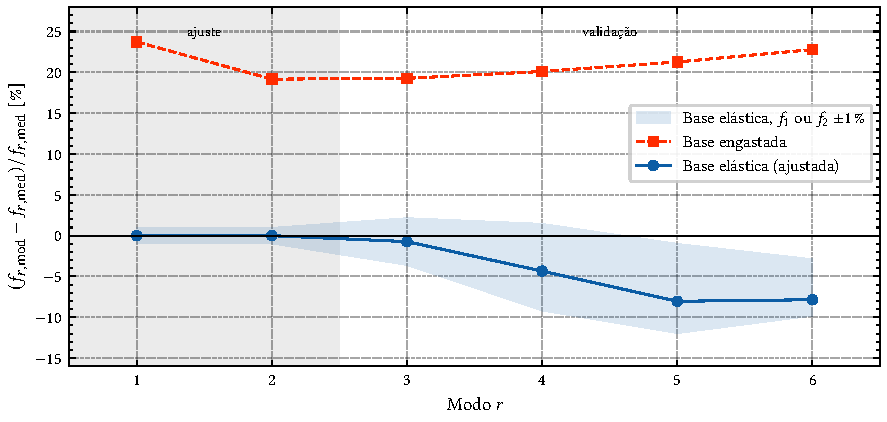
\includegraphics[width=\textwidth]{validacao.pdf}
    \caption{Erro relativo das frequências previstas pelos dois modelos. A faixa azul
        mostra a variação do erro da base elástica quando o ajuste é refeito com $f_1$
        ou $f_2$ alteradas em $\pm\SI{1}{\percent}$.}
    \label{fig:validacao}
\end{figure}

\begin{table}[htbp]
    \centering
    \caption{Sensibilidade do ajuste: rigidezes e erros de validação [\si{\percent}]
        quando $f_1$ ou $f_2$ é alterada em $\pm\SI{1}{\percent}$ antes do ajuste.}
    \label{tab:sensibilidade}
    \begin{tabular}{l rr rrrr}
        \toprule
        Perturbação & $\kappa_R$ & $\kappa_L$ & $e_3$ & $e_4$ & $e_5$ & $e_6$ \\
        \midrule
        Nenhuma     & \vkapR     & \vkapL     & \num{-0.7} & \num{-4.3} & \num{-8.0} & \num{-7.8} \\
        \linhas{sensibilidade}
        \bottomrule
    \end{tabular}
\end{table}

A base elástica reduz o erro do modo 3 de \SI{+19.3}{\percent} para
\SI{-0.7}{\percent} e o do modo 4 de \SI{+20.1}{\percent} para \SI{-4.3}{\percent}.
Nos modos 5 e 6 o erro cai de cerca de \SI{+22}{\percent} para cerca de
\SI{-8}{\percent}. Considerando a sensibilidade da Tabela~\ref{tab:sensibilidade}, os
erros dos modos 3 e 4 são compatíveis com zero para variações de \SI{1}{\percent} nas
frequências de ajuste, comparáveis, por exemplo, ao efeito da massa do acelerômetro
ou à diferença entre os dois ensaios. Já os modos 5 e 6 ficam abaixo do medido em
todos os casos (de \SI{-1}{\percent} a \SI{-12}{\percent}): o modelo ajustado é
flexível demais nos modos altos.

A Figura~\ref{fig:frf_martelo_modelos} compara as FRFs. Com a base elástica, as posições
dos três primeiros picos e o nível da FRF em baixa frequência coincidem com os
medidos, e a altura dos picos 1 e 2, calculada com os $\zeta_r$ do martelo, é da mesma
ordem da medida. O pico 3 do modelo elástico quase não aparece, porque sua constante
modal é praticamente nula (Tabela~\ref{tab:sinais}). A partir do modo 4 os picos do modelo ficam à esquerda dos medidos, como na
Tabela~\ref{tab:validacao}. No \emph{shaker} (Figura~\ref{fig:frf_shaker_modelos}), o
modelo elástico se aproxima dos dois primeiros picos, enquanto os modos 3 e 4 medidos
ficam acima até do engaste, coerente com a restrição na ponta discutida na
Seção~\ref{sec:comparacao_ensaios}. Pela mesma razão, o nível medido em baixa
frequência fica mais perto do modelo engastado: a ligação com o \emph{shaker}
enrijece a ponta. Os picos do \emph{shaker} são mais baixos que os do modelo porque a
varredura não amostra o topo dos picos estreitos.

\begin{figure}[htbp]
    \centering
    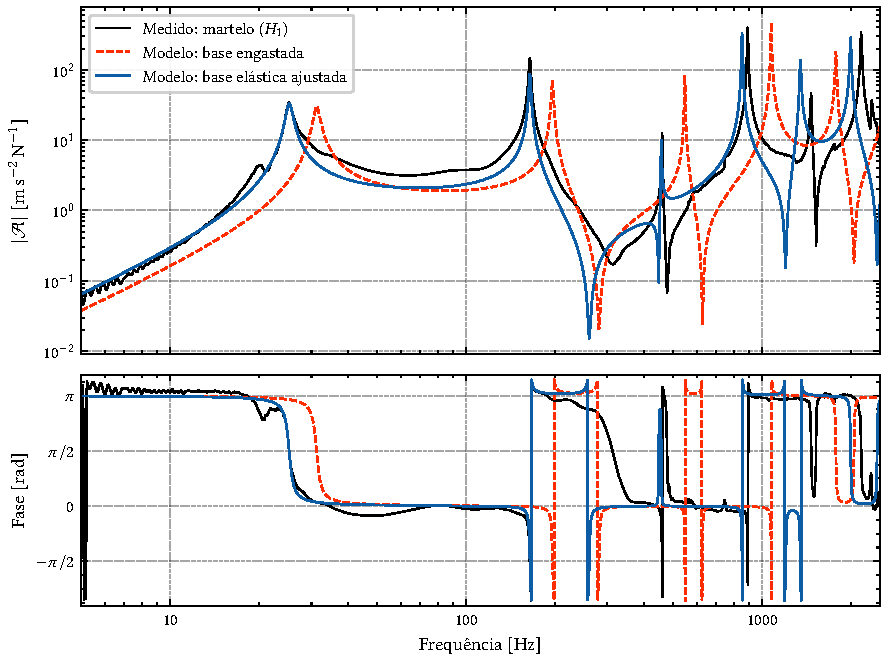
\includegraphics[width=\textwidth]{frf_martelo_modelos.pdf}
    \caption{FRF do ensaio com martelo comparada às acelerâncias analíticas
        \eqref{eq:acelerancia} com base engastada e com base elástica ajustada, ambas com
        os $\zeta_r$ identificados no martelo.}
    \label{fig:frf_martelo_modelos}
\end{figure}

\begin{figure}[htbp]
    \centering
    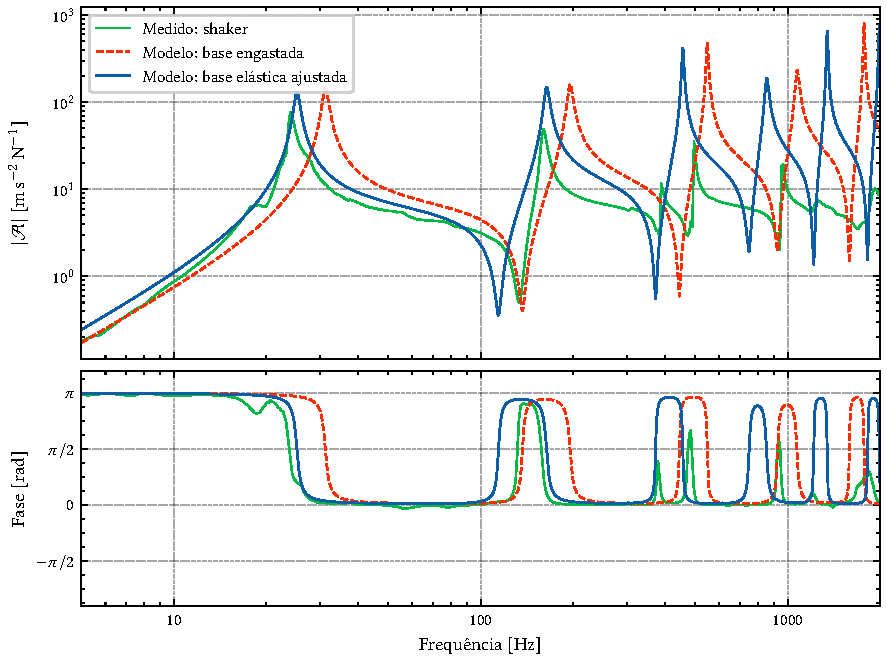
\includegraphics[width=\textwidth]{frf_shaker_modelos.pdf}
    \caption{FRF pontual do ensaio com \emph{shaker} comparada às acelerâncias
        analíticas em $x_i = x_e = L$, com os $\zeta_r$ identificados no
        \emph{shaker}.}
    \label{fig:frf_shaker_modelos}
\end{figure}

\subsubsection{Formas modais e sinais das constantes modais}

A Figura~\ref{fig:modos} mostra os quatro primeiros modos normalizados dos dois
modelos. Com a base elástica, a base gira em todos os modos e passa a transladar nos
modos 3 e 4, e os nós se deslocam em direção à base. Isso altera o sinal da constante
modal $W_r(x_e)W_r(x_i)$ em alguns modos, que pode ser comparado com a fase medida na
ressonância (Tabela~\ref{tab:sinais}). O engaste reproduz o sinal medido nos seis
modos. O modelo elástico acerta os modos 1, 2, 4 e 6, mas erra os modos 3 e 5. No modo
3, o ponto de impacto fica perto de um nó nos dois modelos (em \SI{0.217}{\meter} no
engaste e em \SI{0.196}{\meter} na base elástica), e a constante modal é a menor de
todas, o que explica o pico fraco desse modo; um pequeno deslocamento do nó basta para
trocar o sinal, de modo que esse desacordo pesa pouco. No modo
5, porém, a diferença é clara: o engaste prevê constante positiva, como a medida, e a
base elástica, negativa.

\begin{figure}[htbp]
    \centering
    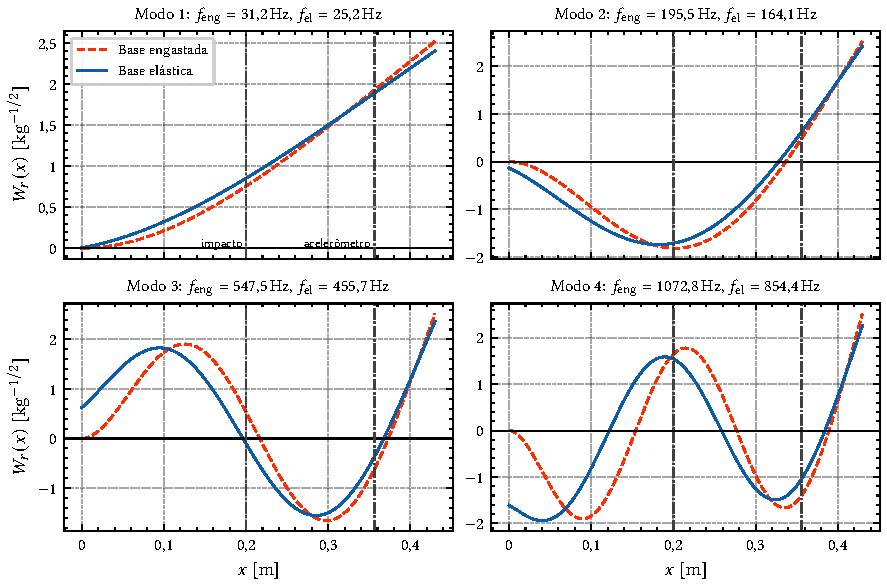
\includegraphics[width=\textwidth]{modos.pdf}
    \caption{Quatro primeiros modos normalizados pela massa, para a base engastada e
        para a base elástica ajustada, com a convenção $W_r(L) > 0$. As linhas
        traço-ponto marcam o ponto de impacto ($x = \SI{0.200}{\meter}$) e o
        acelerômetro ($x = \SI{0.356}{\meter}$).}
    \label{fig:modos}
\end{figure}

\begin{table}[htbp]
    \centering
    \caption[Fase medida nos picos e sinal das constantes modais]{Fase medida no
        pico de cada modo (martelo) e constante modal
        $W_r(x_e)W_r(x_i)$ [\si{\per\kilo\gram}] prevista pelos dois modelos. Fase
        $+\pi/2$ corresponde a constante positiva.}
    \label{tab:sinais}
    \begin{tabular}{c rc rr}
        \toprule
        Modo & Fase medida [\si{\radian}] & Sinal & Engaste & Base elástica \\
        \midrule
        \linhas{sinais}
        \bottomrule
    \end{tabular}
\end{table}

\subsubsection{Qual condição de contorno é adequada?}

Entre as duas hipóteses pedidas no roteiro, a base elástica é claramente a mais
adequada para prever frequências: com dois parâmetros ajustados aos dois primeiros
modos, ela reduz os erros de cerca de \SI{20}{\percent} para menos de
\SI{1}{\percent} no modo 3 e \SI{4.3}{\percent} no modo 4, e reproduz o nível da FRF
em baixa frequência. O engaste ideal é rígido demais em todos os modos. A rigidez à
rotação da fixação, $k_R \approx \SI{2.8e3}{\newton\meter\per\radian}$, é a parte bem
determinada do ajuste e explica a maior parte da diferença.

O modelo de molas, porém, não explica tudo. Três observações indicam que parte da
discrepância não vem só da fixação: (i) a razão $f_{\mathrm{med}}/f_{\mathrm{eng}}$ é
quase constante nos seis modos (\numrange{0.81}{0.84}, Tabela~\ref{tab:validacao}),
enquanto molas na base afetam modos diferentes de forma diferente; (ii) o modelo
ajustado fica flexível demais nos modos 5 e 6; (iii) os sinais das constantes modais
seguem as formas do engaste, não as da base elástica, no modo 5. Um modelo engastado
com todas as frequências multiplicadas por um único fator de \num{0.83}, equivalente a
reduzir $EI/\rho A$ em \SI{32}{\percent} ou a um comprimento efetivo de
\SI{0.473}{\meter}, reproduziria as seis frequências com erro de no máximo
\SI{2.2}{\percent}. Isso sugere que os parâmetros nominais da viga também merecem
revisão; a própria massa $m_b$ do roteiro é inconsistente com $\rho A L$
(Seção~\ref{sec:parametros}). Separar o efeito da fixação do efeito de $EI/\rho A$
exigiria medir a espessura e a massa da viga e obter a resposta em mais pontos, de
modo a identificar as formas modais, inclusive a rotação e a translação na base.

\FloatBarrier
